%----------------------------------------------------------------------------------------
%	PACKAGES AND OTHER DOCUMENT CONFIGURATIONS
%----------------------------------------------------------------------------------------

\documentclass{article}

%----------------------------------------------------------------------------------------
%	PACKAGES AND OTHER DOCUMENT CONFIGURATIONS
%----------------------------------------------------------------------------------------

\usepackage{amsmath,amsfonts,stmaryrd,amssymb} % Math packages
\usepackage{amsfonts,booktabs,siunitx}
\usepackage{enumerate} % Custom item numbers for enumerations

\usepackage[ruled]{algorithm2e} % Algorithms

\usepackage[framemethod=tikz]{mdframed} % Allows defining custom boxed/framed environments

\usepackage{listings} % File listings, with syntax highlighting
\lstset{
	basicstyle=\ttfamily, % Typeset listings in monospace font
}

%----------------------------------------------------------------------------------------
%	DOCUMENT MARGINS
%----------------------------------------------------------------------------------------

\usepackage{geometry} % Required for adjusting page dimensions and margins

\geometry{
	paper=a4paper, % Paper size, change to letterpaper for US letter size
	top=2.5cm, % Top margin
	bottom=3cm, % Bottom margin
	left=2.5cm, % Left margin
	right=2.5cm, % Right margin
	headheight=14pt, % Header height
	footskip=1.5cm, % Space from the bottom margin to the baseline of the footer
	headsep=1.2cm, % Space from the top margin to the baseline of the header
	%showframe, % Uncomment to show how the type block is set on the page
}

%----------------------------------------------------------------------------------------
%	FONTS
%----------------------------------------------------------------------------------------

\usepackage[utf8]{inputenc} % Required for inputting international characters
\usepackage[T1]{fontenc} % Output font encoding for international characters

\usepackage{XCharter} % Use the XCharter fonts

%----------------------------------------------------------------------------------------
%	COMMAND LINE ENVIRONMENT
%----------------------------------------------------------------------------------------

% Usage:
% \begin{commandline}
%	\begin{verbatim}
%		$ ls
%		
%		Applications	Desktop	...
%	\end{verbatim}
% \end{commandline}

\mdfdefinestyle{commandline}{
	leftmargin=10pt,
	rightmargin=10pt,
	innerleftmargin=15pt,
	middlelinecolor=black!50!white,
	middlelinewidth=2pt,
	frametitlerule=false,
	backgroundcolor=black!5!white,
	frametitle={Command Line},
	frametitlefont={\normalfont\sffamily\color{white}\hspace{-1em}},
	frametitlebackgroundcolor=black!50!white,
	nobreak,
}

% Define a custom environment for command-line snapshots
\newenvironment{commandline}{
	\medskip
	\begin{mdframed}[style=commandline]
}{
	\end{mdframed}
	\medskip
}

%----------------------------------------------------------------------------------------
%	FILE CONTENTS ENVIRONMENT
%----------------------------------------------------------------------------------------

% Usage:
% \begin{file}[optional filename, defaults to "File"]
%	File contents, for example, with a listings environment
% \end{file}

\mdfdefinestyle{file}{
	innertopmargin=1.6\baselineskip,
	innerbottommargin=0.8\baselineskip,
	topline=false, bottomline=false,
	leftline=false, rightline=false,
	leftmargin=2cm,
	rightmargin=2cm,
	singleextra={%
		\draw[fill=black!10!white](P)++(0,-1.2em)rectangle(P-|O);
		\node[anchor=north west]
		at(P-|O){\ttfamily\mdfilename};
		%
		\def\l{3em}
		\draw(O-|P)++(-\l,0)--++(\l,\l)--(P)--(P-|O)--(O)--cycle;
		\draw(O-|P)++(-\l,0)--++(0,\l)--++(\l,0);
	},
	nobreak,
}

% Define a custom environment for file contents
\newenvironment{file}[1][File]{ % Set the default filename to "File"
	\medskip
	\newcommand{\mdfilename}{#1}
	\begin{mdframed}[style=file]
}{
	\end{mdframed}
	\medskip
}

%----------------------------------------------------------------------------------------
%	NUMBERED QUESTIONS ENVIRONMENT
%----------------------------------------------------------------------------------------

% Usage:
% \begin{question}[optional title]
%	Question contents
% \end{question}

\mdfdefinestyle{question}{
	innertopmargin=1.2\baselineskip,
	innerbottommargin=0.8\baselineskip,
	roundcorner=5pt,
	nobreak,
	singleextra={%
		\draw(P-|O)node[xshift=1em,anchor=west,fill=white,draw,rounded corners=5pt]{%
		Question \theQuestion\questionTitle};
	},
}

\newcounter{Question} % Stores the current question number that gets iterated with each new question

% Define a custom environment for numbered questions
\newenvironment{question}[1][\unskip]{
	\bigskip
	\stepcounter{Question}
	\newcommand{\questionTitle}{~#1}
	\begin{mdframed}[style=question]
}{
	\end{mdframed}
	\medskip
}

%----------------------------------------------------------------------------------------
%	WARNING TEXT ENVIRONMENT
%----------------------------------------------------------------------------------------

% Usage:
% \begin{warn}[optional title, defaults to "Warning:"]
%	Contents
% \end{warn}

\mdfdefinestyle{warning}{
	topline=false, bottomline=false,
	leftline=false, rightline=false,
	nobreak,
	singleextra={%
		\draw(P-|O)++(-0.5em,0)node(tmp1){};
		\draw(P-|O)++(0.5em,0)node(tmp2){};
		\fill[black,rotate around={45:(P-|O)}](tmp1)rectangle(tmp2);
		\node at(P-|O){\color{white}\scriptsize\bf !};
		\draw[very thick](P-|O)++(0,-1em)--(O);%--(O-|P);
	}
}

% Define a custom environment for warning text
\newenvironment{warn}[1][Warning:]{ % Set the default warning to "Warning:"
	\medskip
	\begin{mdframed}[style=warning]
		\noindent{\textbf{#1}}
}{
	\end{mdframed}
}

%----------------------------------------------------------------------------------------
%	INFORMATION ENVIRONMENT
%----------------------------------------------------------------------------------------

% Usage:
% \begin{info}[optional title, defaults to "Info:"]
% 	contents
% 	\end{info}

\mdfdefinestyle{info}{%
	topline=false, bottomline=false,
	leftline=false, rightline=false,
	nobreak,
	singleextra={%
		\fill[black](P-|O)circle[radius=0.4em];
		\node at(P-|O){\color{white}\scriptsize\bf i};
		\draw[very thick](P-|O)++(0,-0.8em)--(O);%--(O-|P);
	}
}

% Define a custom environment for information
\newenvironment{info}[1][Info:]{ % Set the default title to "Info:"
	\medskip
	\begin{mdframed}[style=info]
		\noindent{\textbf{#1}}
}{
	\end{mdframed}
}
 % Include the file specifying the document structure and custom commands

\title{CS0424IT - Lecture Notes} % Title of the assignment

\author{Simone La Porta} % Author name

\date{\today} 


\begin{document}
\maketitle
\tableofcontents
\newpage
\section{LIVELLO 2 - VLAN}

Switch (livello data, MAC address) permette di \emphy{segmentare} i domini di broadcast mediante la creazione delle virtual LAN, ovvero un insieme logico di host e device di rete: le VLAN si creano aggiungendo un tag o VLAN id alle porte dello switch, o mappando il mac address dell'host con il VLAN ID.

Ipotizzando di voler restringere la comunicazione ed il dominio di broadcast ad A, B, C. Creiamo una VLAN identificata con ID 100 e associamo i MAC di ABC a quella VLAN (ma non quello di D).

Se A invia un pacchetto all'indirizzo di broadcast esso sara ricevuto solamente da B e C. VLAN = segmentano i domini di broadcast e eliminano il problema di latenza su grosse reti.

\section{Livello 3 di rete: router-gateway}

Cosi come per il livello data ci sono dei dispositivi di rete ad hoc (router-gateway): dispositivi di livello 3 che instradano i dati anche a personal computer che sono connessi su reti diverse.

Switch dispositivo di livello 2 e non sa come dirottare i pacchetti su un'altra rete (instrada solo tramite MAC address e non tramite IP address, il quale appartiene al livello di rete).

Il router riceve il pacchetto dallo switch controlla la sua routing table per capire verso quale delle sue interfacce instradare il pacchetto affinché giunga alla rete di destinazione.

\section{LIVELLO 4 - TRASPORTO}

Livello di trasporto si occupa di instaurare un collegamento tra le applicazioni che sono su computer diversi.

ATTENZIONE: pacchetti possono andare persi, non sempre un problema (ad es parlare al telefono) ma puó essere un problema (operazioni finanziare ecc).

Quindi per alcuni servizi/applicativi é \textbf{INDISPENSABILE} che ci sia un controllo sull'effettiva consegna dei pacchetti.

Livello 4 mette a disposizione due protocolli fondamentali: \textbf{TCP} (transmission control protocol), e \textbf{UDP} (user datagram protocol).

TCP: garantisce controllo sul traffico dei pacchetti e sull'effettiva consegna al ricevente. Più sicuro, TCP è connection oriented cioè prima di iniziare lo scambio fa sì che si instauri un canale di comunicazione tra sorgente e destinatario.
Agisce con un \textbf{three-way handshake}:
\begin{itemize}
  \item client che inizia la connessione invia un pacchetto TCP al server destinatario con il flag SYN abilitato ed un numero di sequenza casuale.
  \item server risponde inviando al client un pacchetto con i flag SYN e ACK abilitati, ed un altro numero di sequenza casuale, mentre l'ACK sarà uguale al precedente Seq+1.
  \item client completa la sincronizzazione inviando un pacchetto ACK ed inviando i numeri Seq, ACK, come fatto dal server (ACK sempre Seq ricevuto +1).
\end{itemize}

UDP invece è protocollo connectionless non ha necessità di instaurare un canale di comunicazione prima di iniziare il flusso. Più snello e veloce per attività che richiedono continuo streaming di dati.

Per capire qual è il processo o servizio destinatario di un determinato pacchetto, il TCP o UDP utilizzano le porte o meglio la coppia IP:PORTA.
Mentre con l'IP si identifica la macchina destinataria la porta da info sul servizio. Ogni servizio attivo su un pc utilizza una porta.

Porte si dividono in WELL KNOWN ports utilizzate per i servizi standard tra 0-1023 (prime 1024).

HIGH ports servizi non standard e comunicazione (1024-65535).

Importante ricordare le well known ports associate ai servizi più noti.
SMTP:25

HTTP:80

SSH:22

POP3:110

IMAP:143

NETBIOS:137,138,139

SFTP:115

HTTPS:443

TELNET:23
FTP:21

RDP:3389

MSSQL:1433

MySQL:3306


Per visualizzare porte in ascolto e le connessioni in corso possibile utilizzare NETSTAT che darà in output info circa i demoni (daemon) in ascolto su PC localmente e le connessioni verso server remoti:

netstat -ano (WIN)
netstat -tunp (LINUX)
netstat -p tcp -p udp (MAC)

\section{LIVELLO 5 - SESSIONE}
Livello di applicazione, si organizzano i dati: si apre una sessione (es ssh) tra utente che intende utilizzare un servizio che è in ascolto su un determinato server, si controlla la durata della sessione e di mantenerla attiva durante il flusso di informazioni (ad esempio cambio ip con vpn).

\section{LIVELLO 6 - PRESENTAZIONE}
Preparazione dei dati per essere presentati agli utenti: concetto di CIFRATURA dei dati.

Su un canale di comunicazione i dati possono transitare in maniera visibile o cifrati (ALGORITMO DI CIFRATURA), in maniera tale da rendere disponibili i dati cifrati.

\section{LIVELLO 7 - APPLICAZIONE}

Livello interagisce direttamente con le applicazioni utilizzate. Protocolli più comuni HTTP, HTTPS (cifrato), DNS (traduce la richiesta di un dominio, basato su UDP), FTP (basato su TCP gestisce trasferimento dati tra host).

DNS fondamentale per funzionamento di internet, www(host).store(subdomain).google(domain).com(toplevel domain).

DHCP permette ai dispositivi di una LAN di ricevere una configurazione di rete.

NAT/PAT: network address translation per far fronte all'esaurimento del IPv4. Da questo momento in poi vi è una distinzione tra ip pubblici (es per andare su internet) e privati (interno della rete locale e non raggiungibili su internet), configurati tramite router.

PAT port address translation, forma specifica di NAT in cui oltre alla traduzione degli indirizzi IP vengono anche tradotte le porte dei dispositivi all'interno della rete locale.

Le porte sono numeri a 16bit associati a ogni connessione e PAT permette a più dispositivi di condividere lo stesso IP pubblico distinguendo le loro connessioni in base alle porte.

Mentre NAT traduce indirizzi ip privati in 1 o più indirizzi ip pubblici, il pat va oltre traducendo anche le porte, consentendo a più dispositivi di condividere lo stesso indirizzo ip pubblico.

\end{document}

% \subsection*{Network topology (\href{https://drive.google.com/file/d/1x9iyKs7IbABJt2Fv5kX3HCtqNRj7SI41/view?usp=sharing}{link to .pkz file})}
% For the creation of this naddresses, as indicated next to each one. 
% They were then connected to SWITCH 1, a Layer 2 device in the ISO/OSI model that 
% connects devices within the same IP network. The same process was mirrored for the 
% other 3 hosts (LAPTOP 3, DESKTOP 2 and LAPTOP 4) and another switch, SWITCH 2. Finally, 
% the two switches were connected to allow communication between all 6 hosts.
%
% The summary diagram of the network topology is shown in \Cref{topology}.
%
% \begin{figure}[b!]
%   \frame{
%   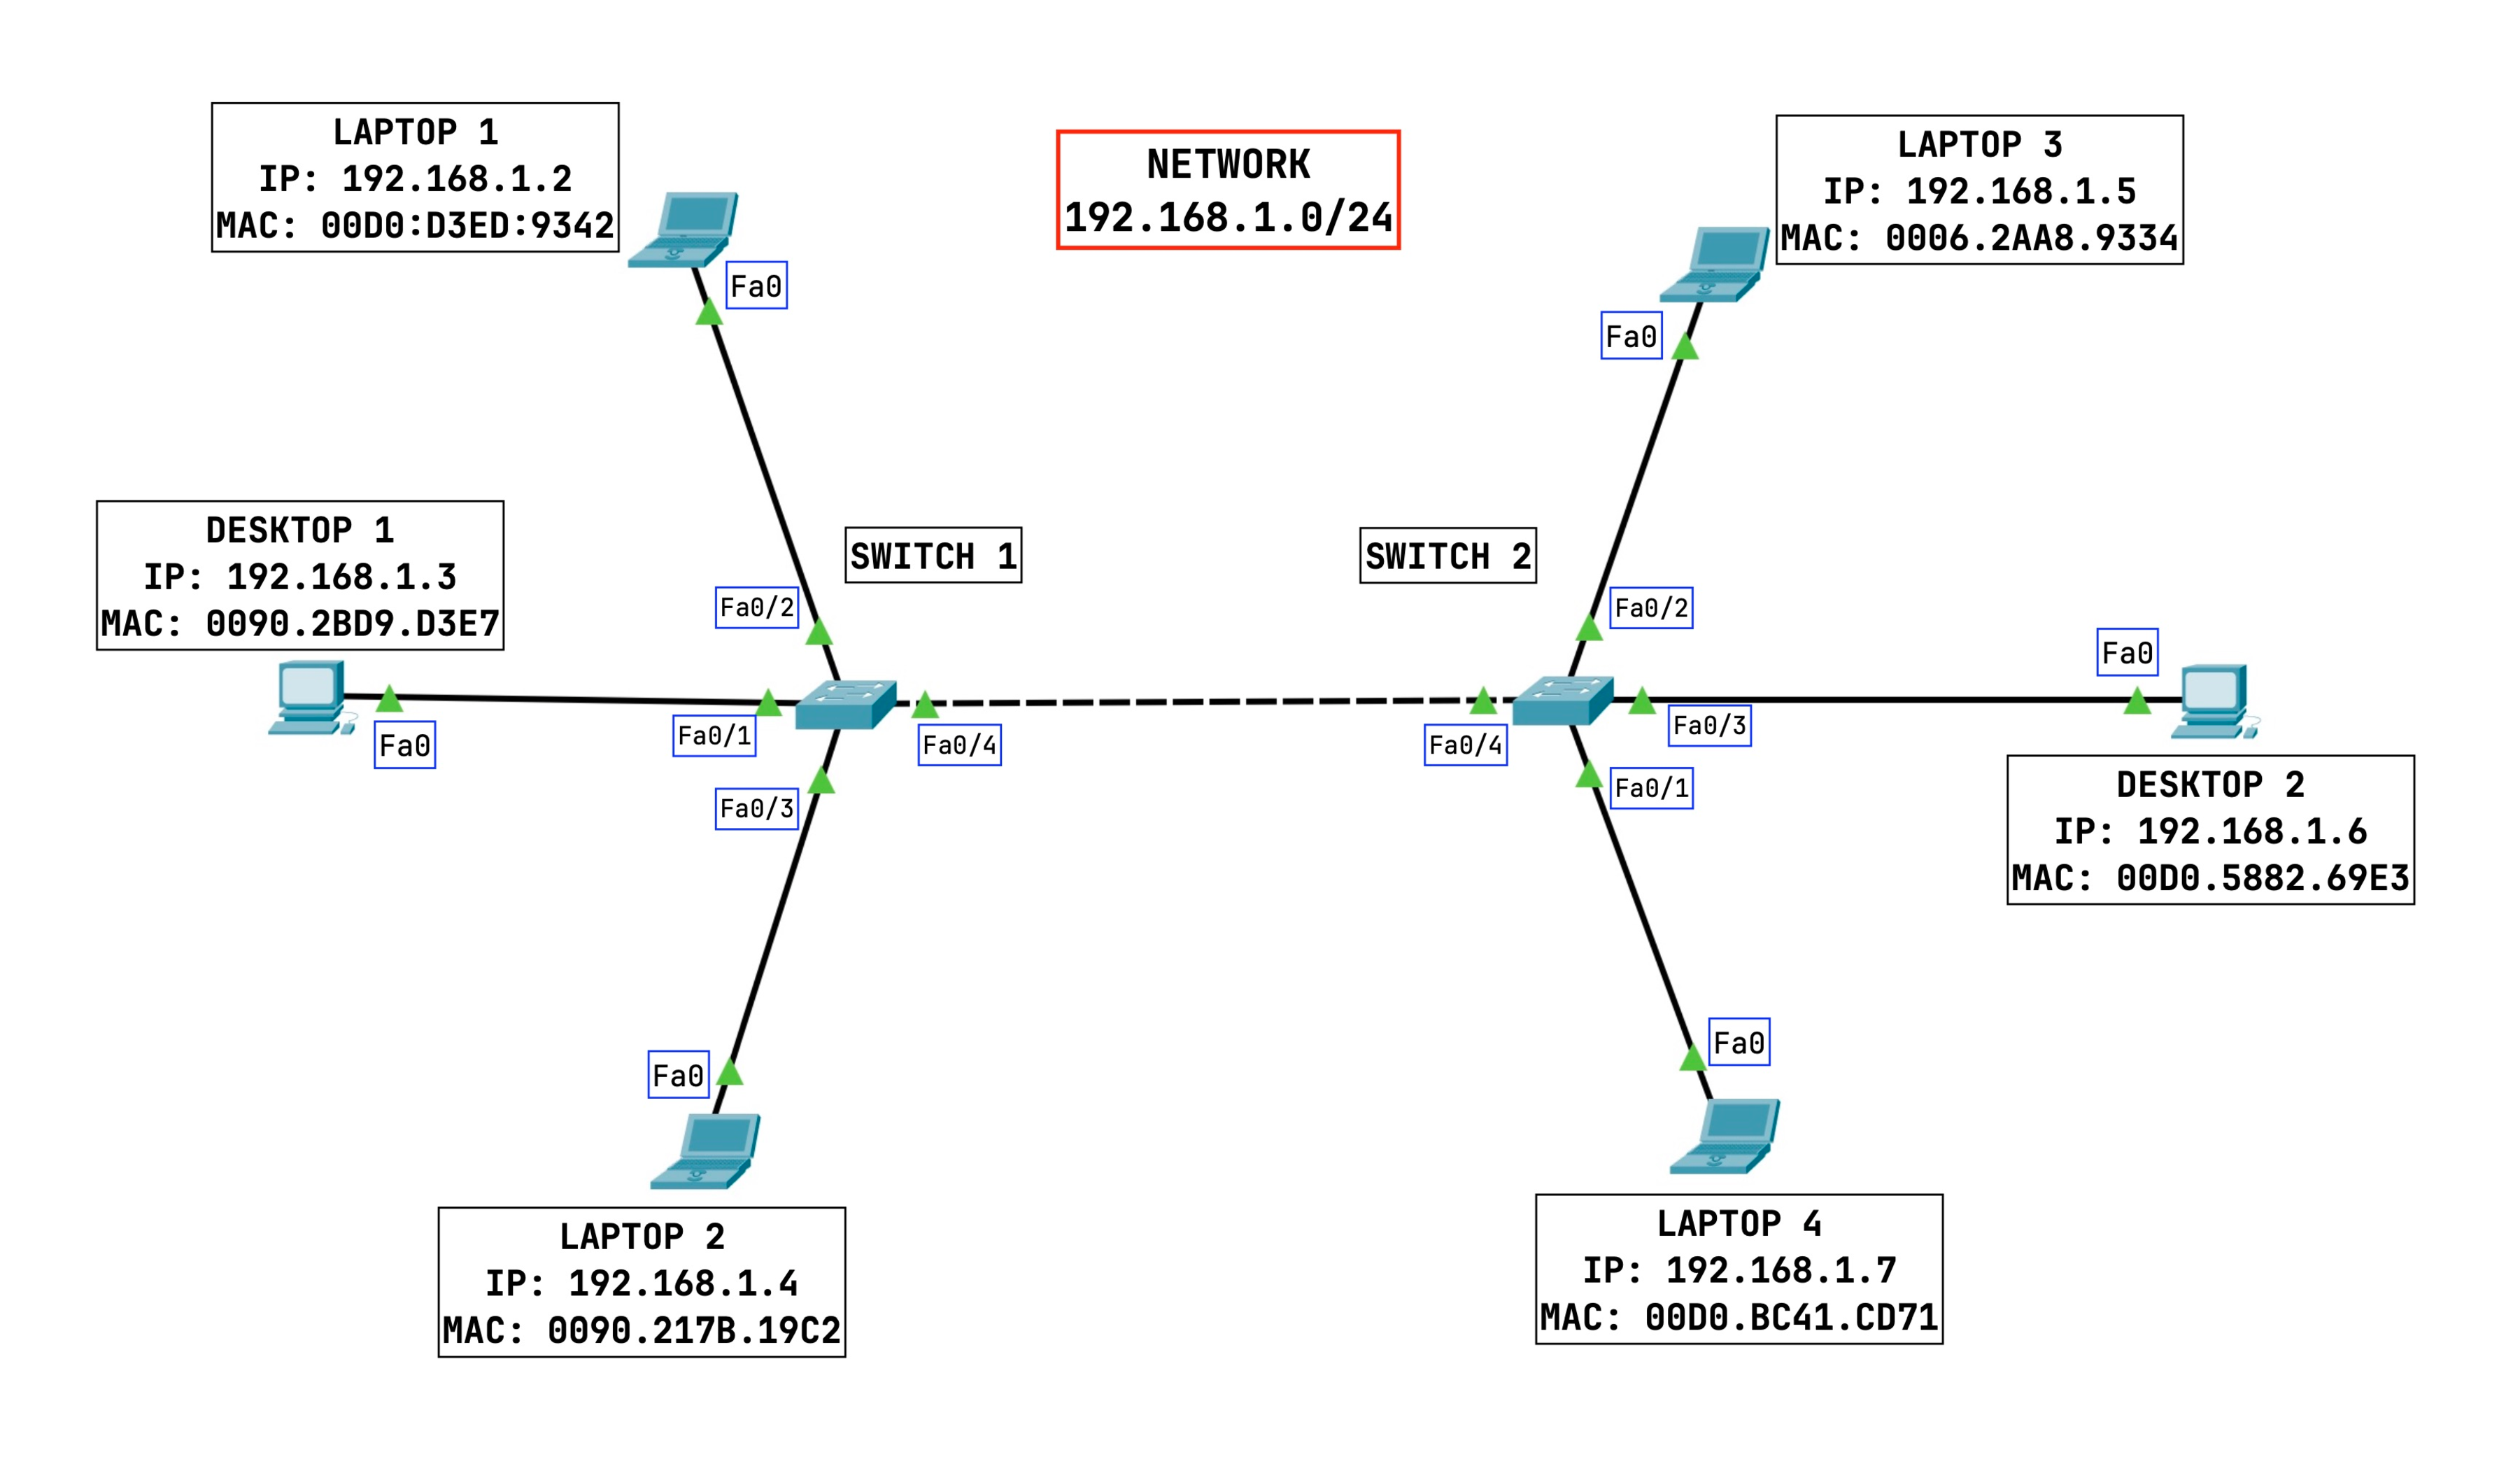
\includegraphics[width=\textwidth,left]{images/network.pdf}
%   }
%   \caption{Summary diagram of the network topology, indicating static IP addresses and 
%   MAC addresses of the devices.}
%   \label{topology}
% \end{figure}
%
% \subsection*{Communication between devices}
% Once the PCs were configured with valid IP addresses from the network, 
% the MAC addresses table of the switches began to fill with the MAC addresses 
% of the devices connected to each switch, as shown in \Cref{mac_tables}. 
% Every switch uses the MAC address table to identify the connected devices, 
% as this table maps MAC addresses to IP addresses.
%
% \begin{figure}
%   \begin{subfigure}{.5\textwidth}
%     \centering
%     \frame{
%     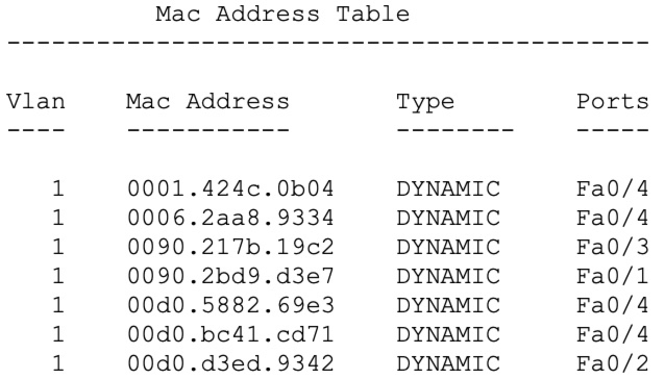
\includegraphics[width=\textwidth]{images/MAC_address_table_switch1.pdf}
%     }
%     \caption{MAC Address Table for SWITCH 1.}
%   \end{subfigure}
%   \begin{subfigure}{.5\textwidth}
%     \centering
%     \frame{
%     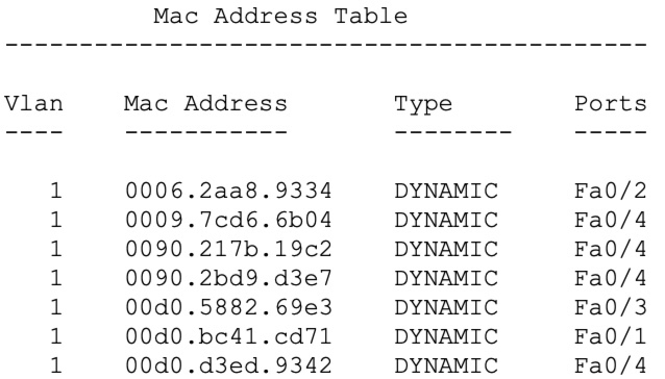
\includegraphics[width=\textwidth]{images/MAC_address_table_switch2.pdf}
%     }
%     \caption{MAC Address Table for SWITCH 2.}
%   \end{subfigure}
%   \caption{MAC Address Tables for the two switches.}
%   \label{mac_tables}
% \end{figure}
%
% To verify the functionality of the network, a \emph{ping} has been sent between each computer to test their connectivity. Pinging allows packets to be sent from one computer to another to verify that they are connected. During the pinging process, the information packet is sent from the sending computer with the destination IP address included. 
% It arrives at the switch, which consults the MAC table to identify the destination IP address and then forwards the packet to the receiving computer.
%
% Proof of connectivity is shown in \Cref{laptop_1,desktop_2}.
%
% \begin{figure}[h!]
%   \begin{subfigure}{.5\textwidth}
%     \centering
%     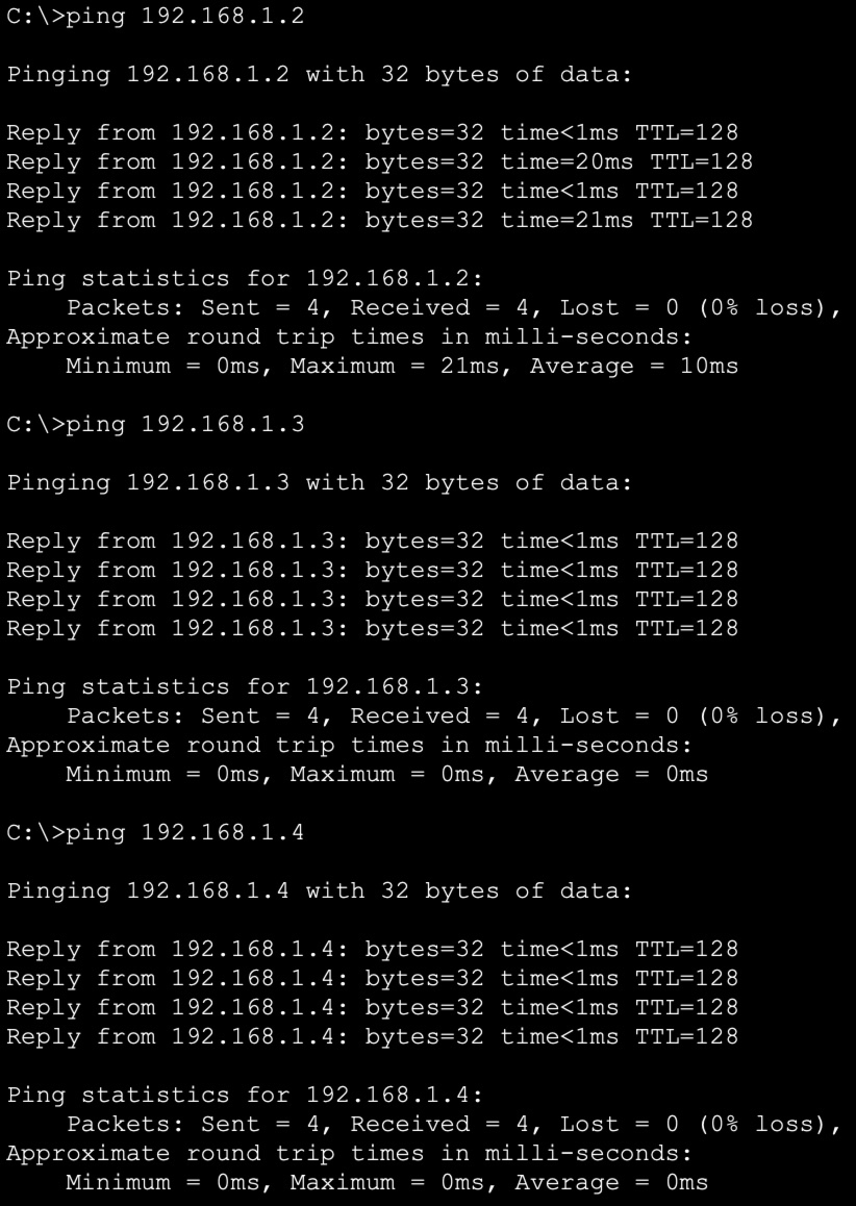
\includegraphics[width=\textwidth]{images/ping_laptop1_to_234.pdf} 
%     %\caption{MAC Address Table for SWITCH 1.}
%   \end{subfigure}
%   \begin{subfigure}{.5\textwidth}
%     \centering
%     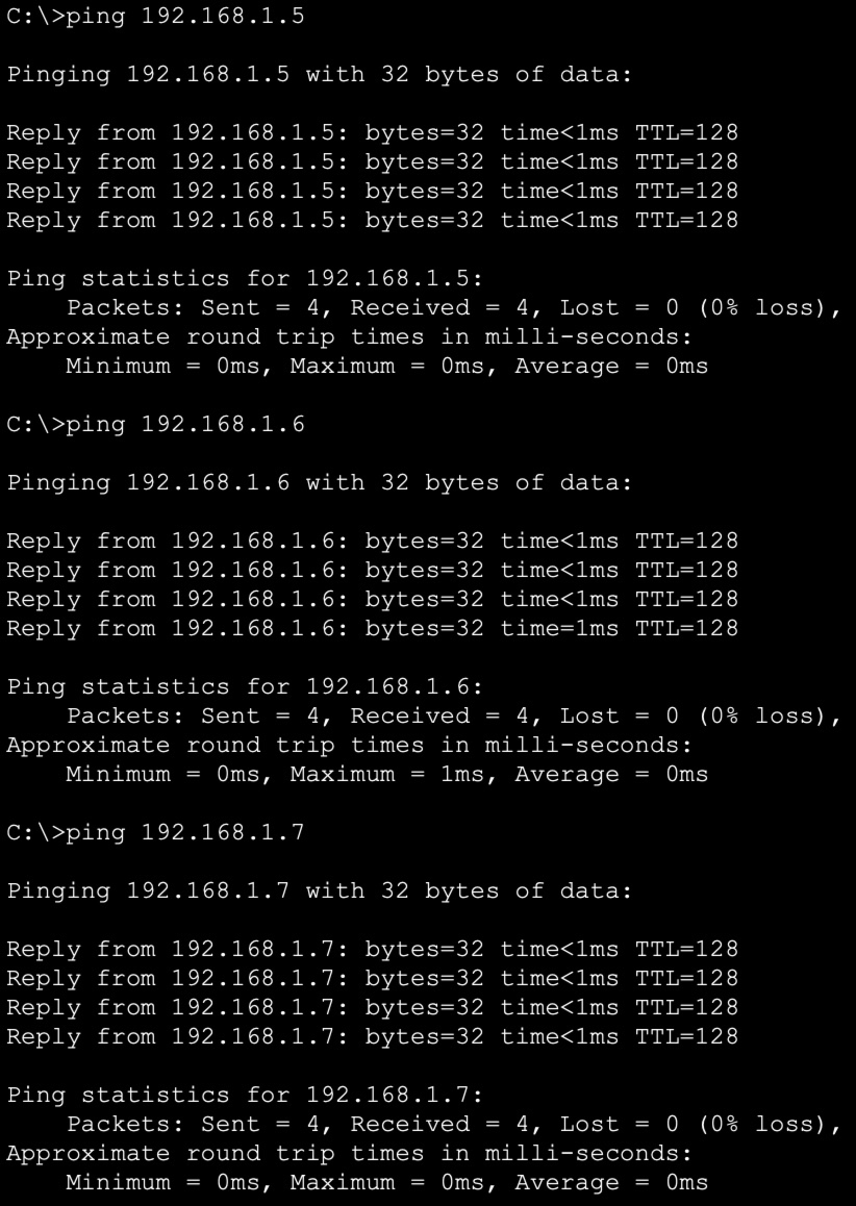
\includegraphics[width=\textwidth]{images/ping_laptop1_to_567.pdf} 
%     %\caption{MAC Address Table for SWITCH 2.}
%   \end{subfigure}
%   \caption{Pinging each network device from LAPTOP 1.}
%   \label{laptop_1}
% \end{figure}
%
%
% \begin{figure}[t!]
%   \begin{subfigure}{.5\textwidth}
%     \centering
%     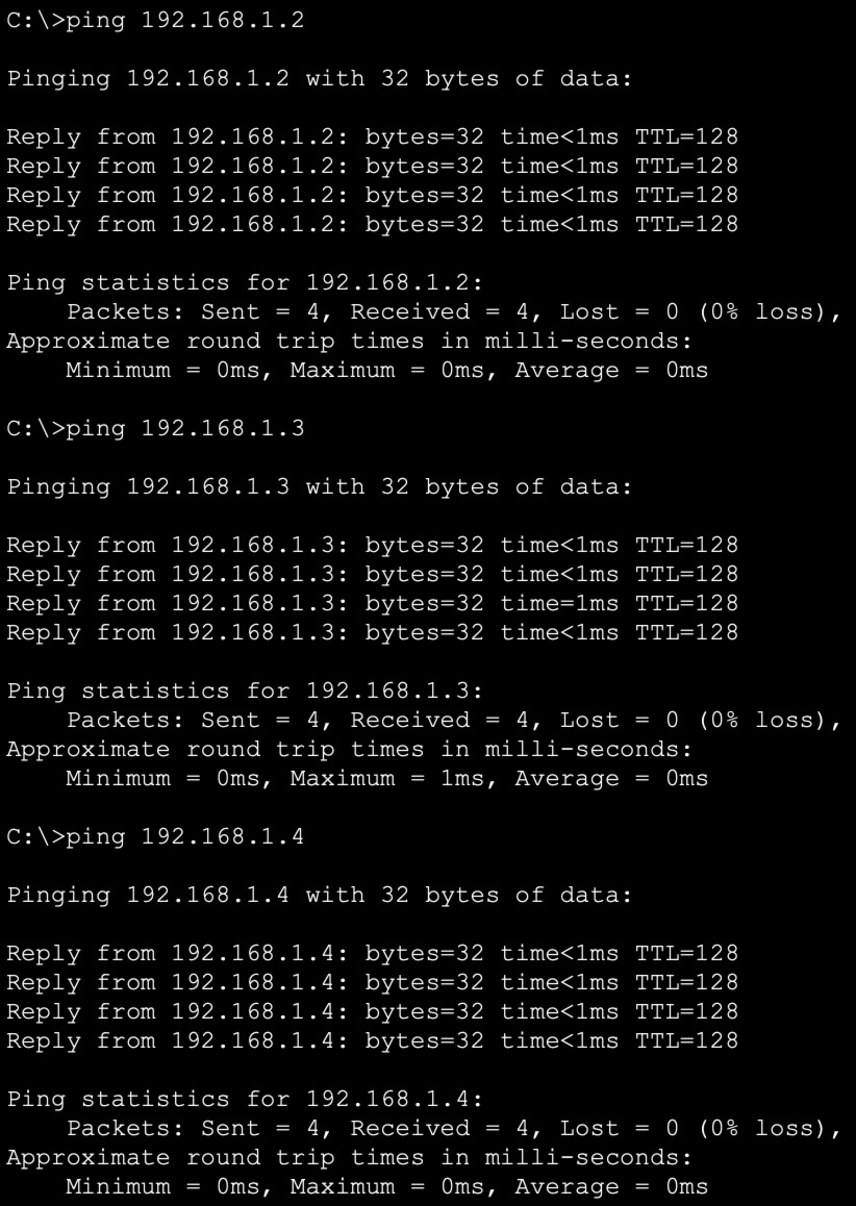
\includegraphics[width=\textwidth]{images/ping_desktop2_to_234.pdf} 
%     %\caption{MAC Address Table for SWITCH 1.}
%   \end{subfigure}
%   \begin{subfigure}{.5\textwidth}
%     \centering
%     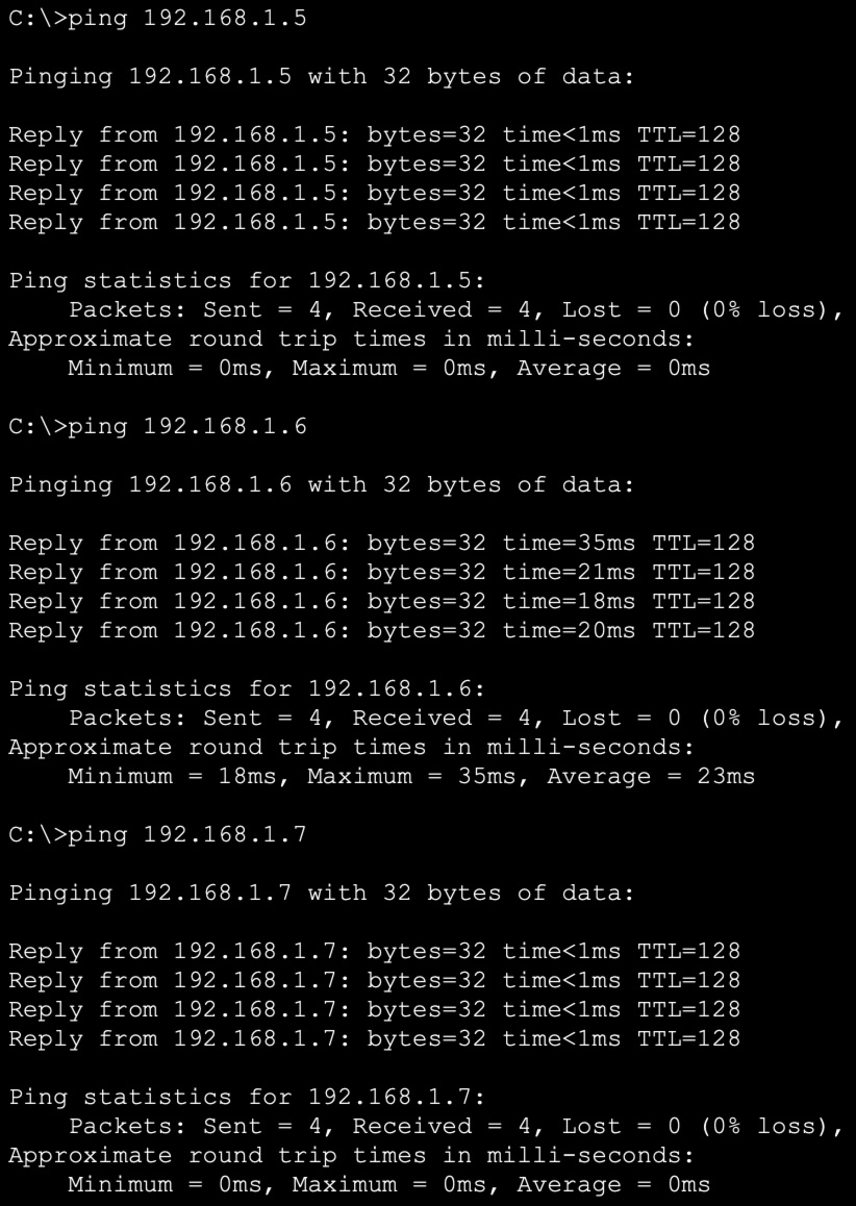
\includegraphics[width=\textwidth]{images/ping_desktop2_to_567.pdf} 
%     %\caption{MAC Address Table for SWITCH 2.}
%   \end{subfigure}
%   \caption{Pinging each network device from DESKTOP 2.}
%   \label{desktop_2}
% \end{figure}
%
%
% \section*{Additional work (\href{https://drive.google.com/file/d/1u0xNbbqKtNcGfd9bF9H4Yti_MXiAxgWF/view?usp=sharing}{link to .pkz file})}
%
% \end{document}
%
%
%
%
% % Math equation/formula
% %\begin{equation}
%
% %\end{equation}
%
% %\begin{info} % Information block
% %	This is an interesting piece of information, to which the reader should pay special attention. Fusce varius orci ac magna dapibus porttitor. In tempor leo a neque bibendum sollicitudin. Nulla pretium fermentum nisi, eget sodales magna facilisis eu. Praesent aliquet nulla ut bibendum lacinia. Donec vel mauris vulputate, commodo ligula ut, egestas orci. Suspendisse commodo odio sed hendrerit lobortis. Donec finibus eros erat, vel ornare enim mattis et.
% %\end{info}
%
%
% % Numbered question, with subquestions in an enumerate environment
% %\begin{question}
% %	Quisque ullamcorper placerat ipsum. Cras nibh. Morbi vel justo vitae lacus tincidunt ultrices. Lorem ipsum dolor sit amet, consectetuer adipiscing elit.
%
% 	% Subquestions numbered with letters
% %	\begin{enumerate}[(a)]
% %		\item Do this.
% %		\item Do that.
% %		\item Do something else.
% %	\end{enumerate}
% %\end{question}
%
%
% %\subsection{Algorithmic issues}
%
%
% %\begin{center}
% %	\begin{minipage}{0.5\linewidth} % Adjust the minipage width to accomodate for the length of algorithm lines
% %		\begin{algorithm}[H]
% %			\KwIn{$(a, b)$, two floating-point numbers}  % Algorithm inputs
% %			\KwResult{$(c, d)$, such that $a+b = c + d$} % Algorithm outputs/results
% %			\medskip
% %			\If{$\vert b\vert > \vert a\vert$}{
% %				exchange $a$ and $b$ \;
% %			}
% %			$c \leftarrow a + b$ \;
% %			$z \leftarrow c - a$ \;
% %			$d \leftarrow b - z$ \;
% %			{\bf return} $(c,d)$ \;
% %			\caption{\texttt{FastTwoSum}} % Algorithm name
% %			\label{alg:fastTwoSum}   % optional label to refer to
% %		\end{algorithm}
% %	\end{minipage}
% %\end{center}
%
%
% % Numbered question, with an optional title
% %\begin{question}[\itshape (with optional title)]
% %	In congue risus leo, in gravida enim viverra id. Donec eros mauris, bibendum vel dui at, tempor commodo augue. In vel lobortis lacus. Nam ornare ullamcorper mauris vel molestie. Maecenas vehicula ornare turpis, vitae fringilla orci consectetur vel. Nam pulvinar justo nec neque egestas tristique. Donec ac dolor at libero congue varius sed vitae lectus. Donec et tristique nulla, sit amet scelerisque orci. Maecenas a vestibulum lectus, vitae gravida nulla. Proin eget volutpat orci. Morbi eu aliquet turpis. Vivamus molestie urna quis tempor tristique. Proin hendrerit sem nec tempor sollicitudin.
% %\end{question}
%
%
% %----------------------------------------------------------------------------------------
% %	PROBLEM 2
% %----------------------------------------------------------------------------------------
%
% %\section{Implementation}
%
%
% % File contents
% %\begin{file}[hello.py]
% %\begin{lstlisting}[language=Python]
% %#! /usr/bin/python
%
% %import sys
% %sys.stdout.write("Hello World!\n")
% %\end{lstlisting}
% %\end{file}
%
%
% % Command-line "screenshot"
% %\begin{commandline}
% %	\begin{verbatim}
% %		$ chmod +x hello.py
% %		$ ./hello.py
% %
% 	%	Hello World!
% 	%\end{verbatim}
% %\end{commandline}
%
%
% % Warning text, with a custom title
% %\begin{warn}[Notice:]
% %  In congue risus leo, in gravida enim viverra id. Donec eros mauris, bibendum vel dui at, tempor commodo augue. In vel lobortis lacus. Nam ornare ullamcorper mauris vel molestie. Maecenas vehicula ornare turpis, vitae fringilla orci consectetur vel. Nam pulvinar justo nec neque egestas tristique. Donec ac dolor at libero congue varius sed vitae lectus. Donec et tristique nulla, sit amet scelerisque orci. Maecenas a vestibulum lectus, vitae gravida nulla. Proin eget volutpat orci. Morbi eu aliquet turpis. Vivamus molestie urna quis tempor tristique. Proin hendrerit sem nec tempor sollicitudin.
% %\end{warn}
